\documentclass[a4paper, font=12pt]{article}
  \usepackage{tikz}
    \usetikzlibrary{shapes.geometric, arrows, positioning}
  
%%%%% flow chart configuration %%%%%
\tikzstyle{main} = [font=\large \ttfamily, minimum width=0.5cm, minimum height=0.5cm, text centered, draw=black, align=center, fill=yellow!10, draw=none]
\tikzstyle{f} = [font=\ttfamily, minimum width=0.5cm, minimum height=0.5cm, text centered, draw=black, align=center, draw=none]
\tikzstyle{other} = [font=\ttfamily, minimum width=0.5cm, minimum height=0.5cm, text centered, draw=black, align=center, draw=none, fill=gray!10]
\tikzstyle{within} = [rectangle, rounded corners, dotted, font=\ttfamily, minimum width=0.5cm, minimum height=0.5cm, text centered, draw=black, align=center]
\tikzstyle{arrow} = [thick,->,>=stealth]

\begin{document}

\begin{itemize}
\item Asterisks indicate main (top-level) functions
\item Arrows indicate functions called
\item Grey boxes indicate functions called from different R scripts
\item Dotted nodes indicate nested functions
\end{itemize}

\vspace{5em}

%%%%%%%%%%%%%%%
% bootstrap.R %
%%%%%%%%%%%%%%%
\begin{figure}[h]
\centering
  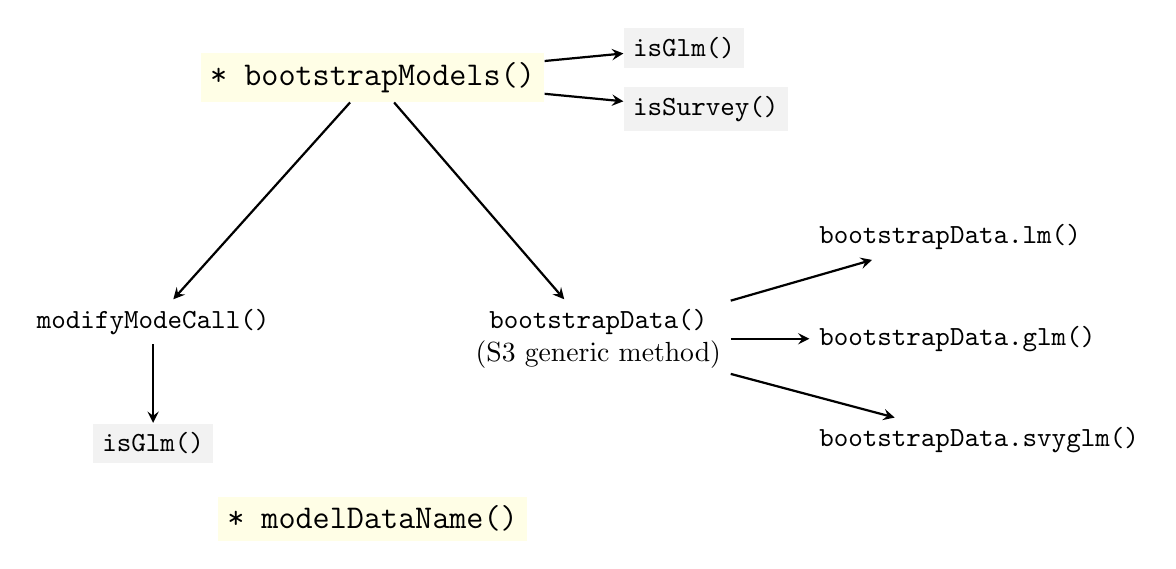
\begin{tikzpicture}
    \node(1)[main]{* bootstrapModels()};
      \node(1-a)[f, below right=of 1, xshift=-2cm, yshift=-1.5cm]{bootstrapData() \\ \normalfont (S3 generic method)};
        \node(1-a-a)[f, above right=of 1-a, yshift=-.5cm]{bootstrapData.lm()};
        \node(1-a-b)[f, right=of 1-a]{bootstrapData.glm()};
        \node(1-a-c)[f, below right=of 1-a, yshift=.5cm]{bootstrapData.svyglm()};
      \node(1-b)[f, below left=of 1, xshift=2cm, yshift=-1.5cm]{modifyModeCall()};
        \node(1-b-a)[other, below=of 1-b]{isGlm()};
      \node(1-c)[other, above right=of 1, yshift=-1.2cm]{isGlm()};
      \node(1-d)[other, below right=of 1, yshift=1.2cm]{isSurvey()};
    \node(2)[main, below=of 1, yshift=-4cm]{* modelDataName()};
    \draw[arrow](1)--(1-a);
    \draw[arrow](1)--(1-b);
    \draw[arrow](1)--(1-c);
    \draw[arrow](1)--(1-d);
    \draw[arrow](1-a)--(1-a-a);
    \draw[arrow](1-a)--(1-a-b);
    \draw[arrow](1-a)--(1-a-c);
    \draw[arrow](1-b)--(1-b-a);
  \end{tikzpicture}
  \caption{\texttt{bootstrap.R}}
\end{figure}

%%%%%%%%%%%%%%%%%%%
% bootstrapCoef.R %
%%%%%%%%%%%%%%%%%%%
\begin{figure}
\centering
  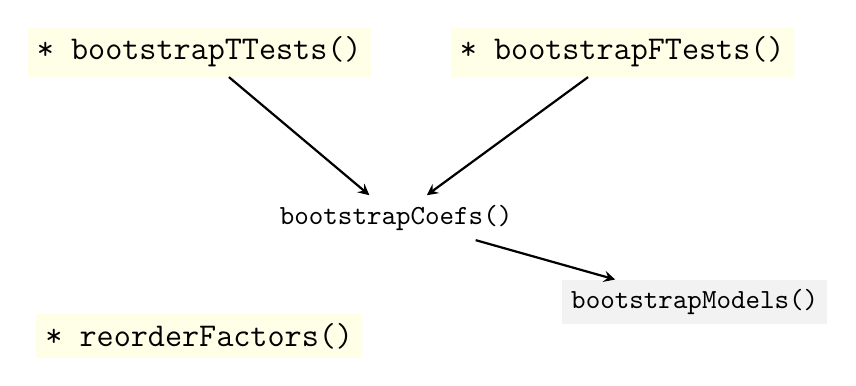
\begin{tikzpicture}
    \node(1)[main]{* bootstrapTTests()};
    \node(2)[main, right=of 1]{* bootstrapFTests()};
      \node(12-a)[f, below=of 1, xshift=2.5cm, yshift=-0.5cm]{bootstrapCoefs()};
        \node(12-a-a)[other, below right=of 12-a, xshift=-0.5cm, yshift=0.5cm]{bootstrapModels()};
    \node(3)[main, below=of 1, yshift=-2cm]{* reorderFactors()};
    \draw[arrow](1)--(12-a);
    \draw[arrow](2)--(12-a);
    \draw[arrow](12-a)--(12-a-a);
  \end{tikzpicture}
  \caption{\texttt{bootstrapCoef.R}}
\end{figure}

%%%%%%%%%%%%%%%%%
% factorMeans.R %
%%%%%%%%%%%%%%%%%
\begin{figure}
\centering
  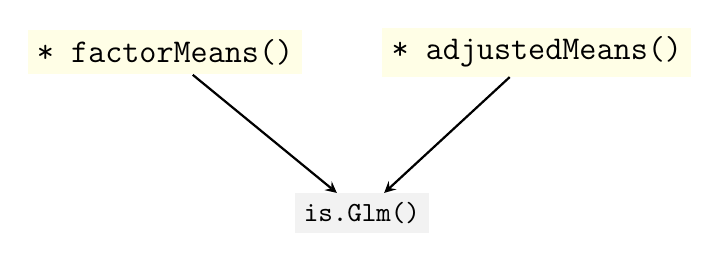
\begin{tikzpicture}
    \node(1)[main]{* factorMeans()};
    \node(2)[main, right=of 1]{* adjustedMeans()};
      \node(12-a)[other, below=of 1, xshift=2.5cm, yshift=-0.5cm]{is.Glm()};     
    \draw[arrow](1)--(12-a);
    \draw[arrow](2)--(12-a);
  \end{tikzpicture}
  \caption{\texttt{factorMeans.R}}
\end{figure}

%%%%%%%%%%%%%%%%%%%%
% histogramArray.R %
%%%%%%%%%%%%%%%%%%%%
\begin{figure}
\centering
  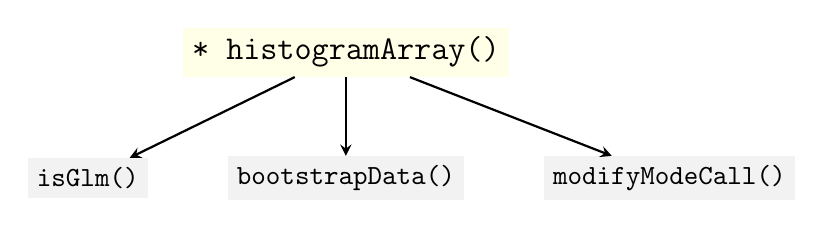
\begin{tikzpicture}
    \node(1)[main]{* histogramArray()};
      \node(1-b)[other, below=of 1]{bootstrapData()};
      \node(1-a)[other, left=of 1-b]{isGlm()};
      \node(1-c)[other, right=of 1-b]{modifyModeCall()};
    \draw[arrow](1)--(1-a);
    \draw[arrow](1)--(1-b);
    \draw[arrow](1)--(1-c);
  \end{tikzpicture}
  \caption{\texttt{histogramArray.R}}
\end{figure}

%%%%%%%%%%%%%%%%%%%
% iNZightQQplot.R %
%%%%%%%%%%%%%%%%%%%
\begin{figure}
\centering
  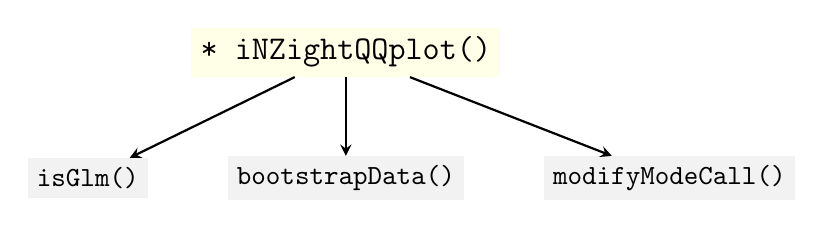
\begin{tikzpicture}
    \node(1)[main]{* iNZightQQplot()};
      \node(1-b)[other, below=of 1]{bootstrapData()};
      \node(1-a)[other, left=of 1-b]{isGlm()};
      \node(1-c)[other, right=of 1-b]{modifyModeCall()};
    \draw[arrow](1)--(1-a);
    \draw[arrow](1)--(1-b);
    \draw[arrow](1)--(1-c);
  \end{tikzpicture}
  \caption{\texttt{iNZightQQplot.R}}
\end{figure}

%%%%%%%%%%%%%%%%%%%
% moe-multicomp.R %
%%%%%%%%%%%%%%%%%%%
\begin{figure}
\centering
  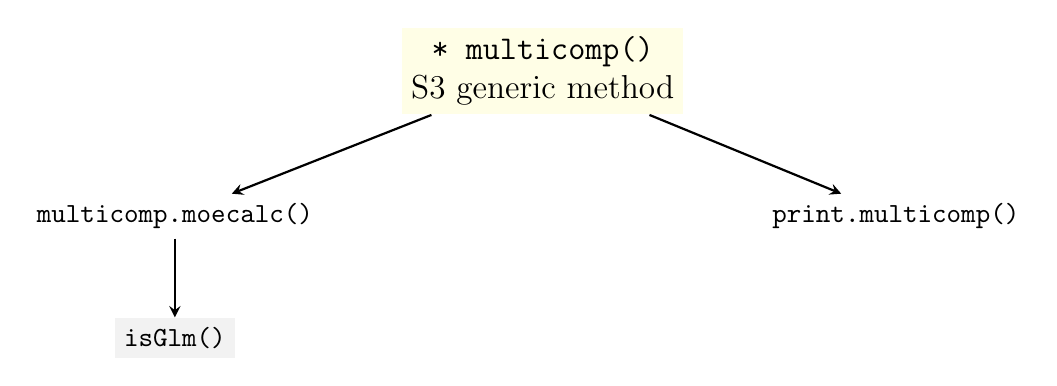
\begin{tikzpicture}
    \node(1)[main]{* multicomp() \\ \normalfont S3 generic method};
      \node(1-a)[f, below left=of 1]{multicomp.moecalc()};
      \node(1-b)[f, below right=of 1]{print.multicomp()};
        \node(1-a-a)[other, below=of 1-a]{isGlm()};
    \draw[arrow](1)--(1-a);
    \draw[arrow](1)--(1-b);
    \draw[arrow](1-a)--(1-a-a);
  \end{tikzpicture}
  \caption{\texttt{moe-multicomp.R}}
\end{figure}

%%%%%%%%%%%%%
% moecalc.R %
%%%%%%%%%%%%%
\begin{figure}
\centering
  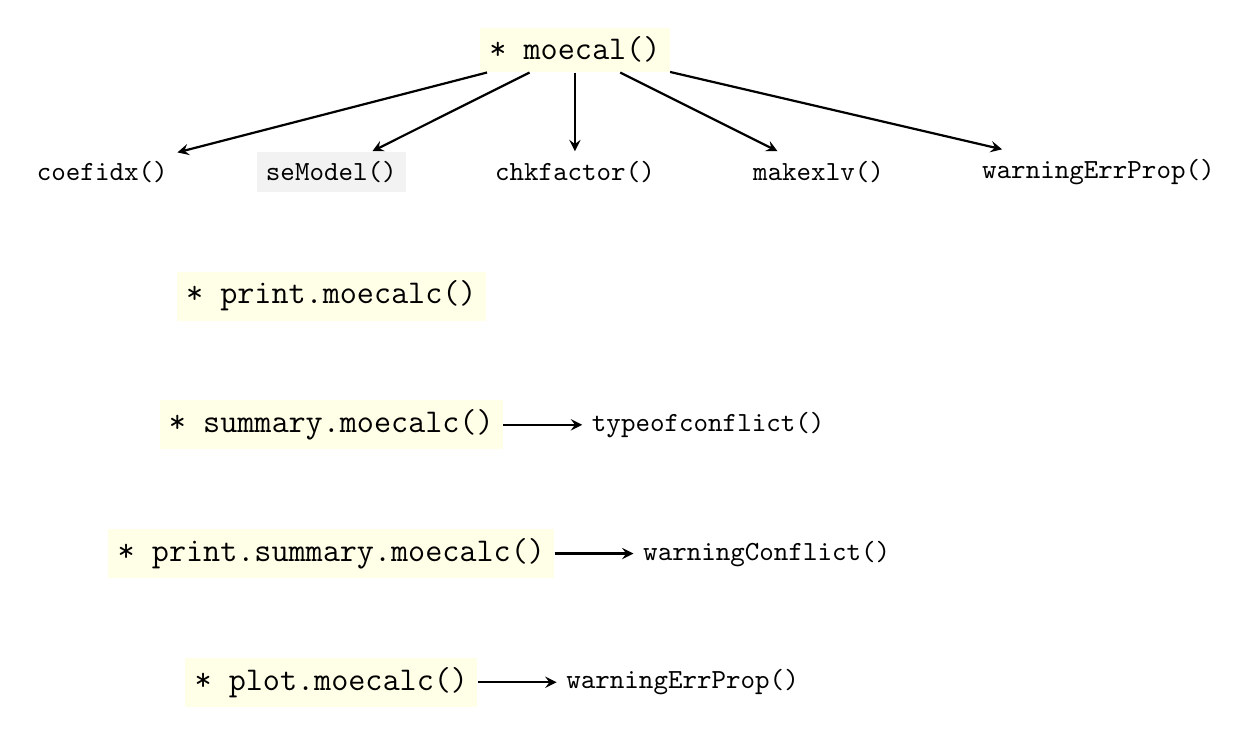
\begin{tikzpicture}
    \node(1)[main]{* moecal()};
      \node(1-c)[f, below=of 1]{chkfactor()};
      \node(1-b)[other, left=of 1-c]{seModel()};
      \node(1-a)[f, left=of 1-b]{coefidx()};
      \node(1-d)[f, right=of 1-c]{makexlv()};
      \node(1-e)[f, right=of 1-d]{warningErrProp()};
    \node(2)[main, below=of 1-b]{* print.moecalc()};
    \node(3)[main, below=of 2]{* summary.moecalc()};
      \node(3-a)[f, right=of 3]{typeofconflict()};
    \node(4)[main, below=of 3]{* print.summary.moecalc()};
      \node(4-a)[f, right=of 4]{warningConflict()};
    \node(5)[main, below=of 4]{* plot.moecalc()};
      \node(5-a)[f, right=of 5]{warningErrProp()};
    \draw[arrow](1)--(1-a);
    \draw[arrow](1)--(1-b);
    \draw[arrow](1)--(1-c);
    \draw[arrow](1)--(1-d);
    \draw[arrow](1)--(1-e);
    \draw[arrow](3)--(3-a);
    \draw[arrow](4)--(4-a);
    \draw[arrow](5)--(5-a);
  \end{tikzpicture}
  \caption{\texttt{moecalc.R}}
\end{figure}

%%%%%%%%%%%%%%%%%%%%%
% partialResidual.R %
%%%%%%%%%%%%%%%%%%%%%
\begin{figure}
\centering
  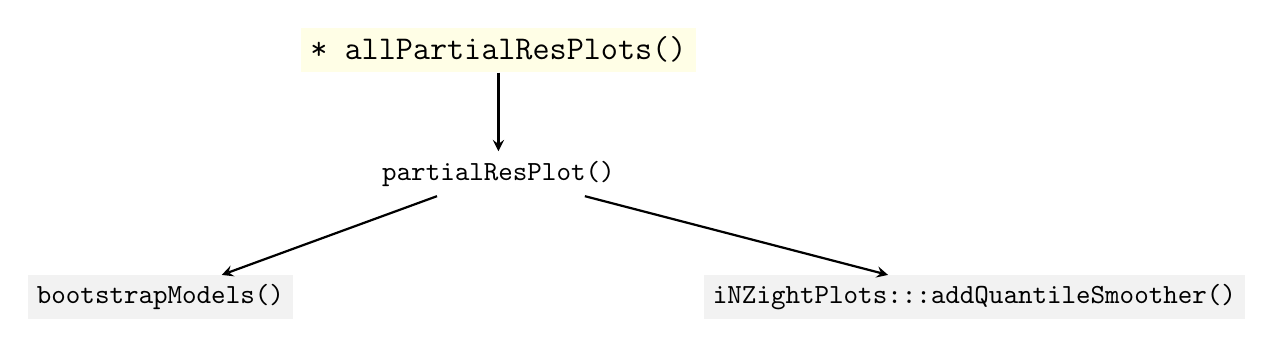
\begin{tikzpicture}
    \node(1)[main]{* allPartialResPlots()};
      \node(1-a)[f, below=of 1]{partialResPlot()};
        \node(1-a-a)[other, below left=of 1-a]{bootstrapModels()};
        \node(1-a-b)[other, below right=of 1-a]{iNZightPlots:::addQuantileSmoother()};
    \draw[arrow](1)--(1-a);
    \draw[arrow](1-a)--(1-a-a);
    \draw[arrow](1-a)--(1-a-b);
  \end{tikzpicture}
  \caption{\texttt{partialResidual.R}}
\end{figure}

%%%%%%%%%%%%%
% plotlm6.R %
%%%%%%%%%%%%%
\begin{figure}
\centering
  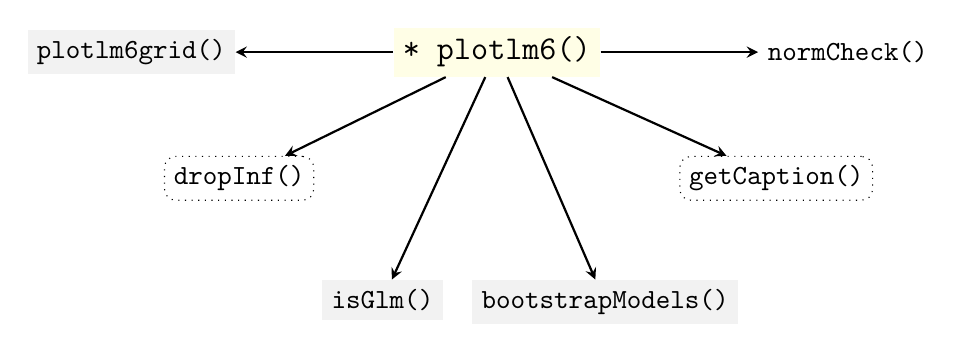
\begin{tikzpicture}
    \node(1)[main]{* plotlm6()};
      \node(1-a)[other, left=of 1, xshift=-1cm]{plotlm6grid()};
      \node(1-b)[within, below left=of 1]{dropInf()};
      \node(1-c)[other, below right=of 1-b, xshift=1cm]{bootstrapModels()};
      \node(1-e)[within, below right=of 1]{getCaption()};
      \node(1-d)[other, below left=of 1-e, xshift=-2cm]{isGlm()};
      \node(1-f)[f, right=of 1, xshift=1cm]{normCheck()};
    \draw[arrow](1)--(1-a);
    \draw[arrow](1)--(1-b);
    \draw[arrow](1)--(1-c);
    \draw[arrow](1)--(1-d);
    \draw[arrow](1)--(1-e);
    \draw[arrow](1)--(1-f);
  \end{tikzpicture}
  \caption{\texttt{plotlm6.R}}
\end{figure}

%%%%%%%%%%%%%%%%%
% plotlm6grid.R %
%%%%%%%%%%%%%%%%%
\begin{figure}
\centering
  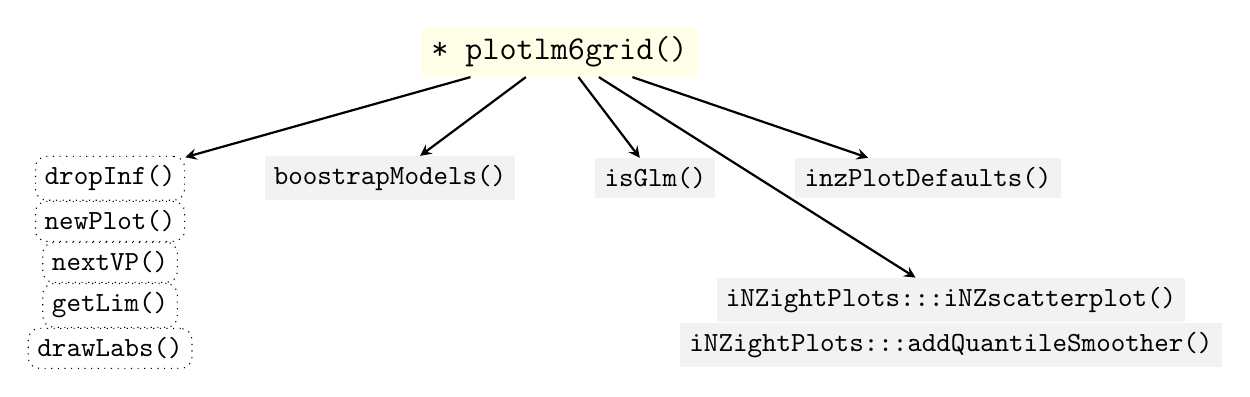
\begin{tikzpicture}
    \node(1)[main]{* plotlm6grid()};
      \node(1-a)[within, below left=of 1, xshift=-2cm]{dropInf()};
        \node(1-a-a)[within, below=of 1-a, yshift=1cm]{newPlot()};
        \node(1-a-b)[within, below=of 1-a-a, yshift=1cm]{nextVP()};
        \node(1-a-c)[within, below=of 1-a-b, yshift=1cm]{getLim()};
        \node(1-a-d)[within, below=of 1-a-c, yshift=1cm]{drawLabs()};
      \node(1-b)[other, right=of 1-a]{boostrapModels()};
      \node(1-c)[other, right=of 1-b]{isGlm()};
      \node(1-d)[other, right=of 1-c]{inzPlotDefaults()};
      \node(1-e)[other, below right=of 1-c, xshift=-1cm]{iNZightPlots:::iNZscatterplot()};
      \node(1-f)[other, below=of 1-e, yshift=1cm]{iNZightPlots:::addQuantileSmoother()};
    \draw[arrow](1)--(1-a);
    \draw[arrow](1)--(1-b);
    \draw[arrow](1)--(1-c);
    \draw[arrow](1)--(1-d);
    \draw[arrow](1)--(1-e);
  \end{tikzpicture}
  \caption{\texttt{plotlm6grid.R}}
\end{figure}

%%%%%%%%%%%%%%%%%
% ses.moecalc.R %
%%%%%%%%%%%%%%%%%
\begin{figure}
\centering
  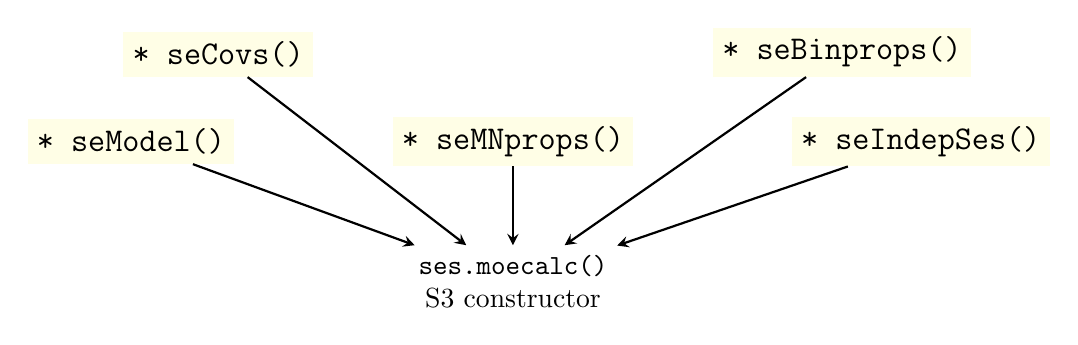
\begin{tikzpicture}
      \node(12345-a)[f]{ses.moecalc() \\ \normalfont S3 constructor};
    \node(3)[main, above=of 12345-a]{* seMNprops()};
    \node(2)[main, above left=of 3, yshift=-0.5cm]{* seCovs()};
    \node(1)[main, left=of 3, xshift=-1cm]{* seModel()};
    \node(4)[main, above right=of 3, yshift=-0.5cm]{* seBinprops()};
    \node(5)[main, right=of 3, xshift=1cm]{* seIndepSes()};
    \draw[arrow](1)--(12345-a);
    \draw[arrow](2)--(12345-a);
    \draw[arrow](3)--(12345-a);
    \draw[arrow](4)--(12345-a);
    \draw[arrow](5)--(12345-a);
  \end{tikzpicture}
  \caption{\texttt{ses.moecalc.R}}
\end{figure}

%%%%%%%%%%%%%
% summary.R %
%%%%%%%%%%%%%
\begin{figure}
\centering
  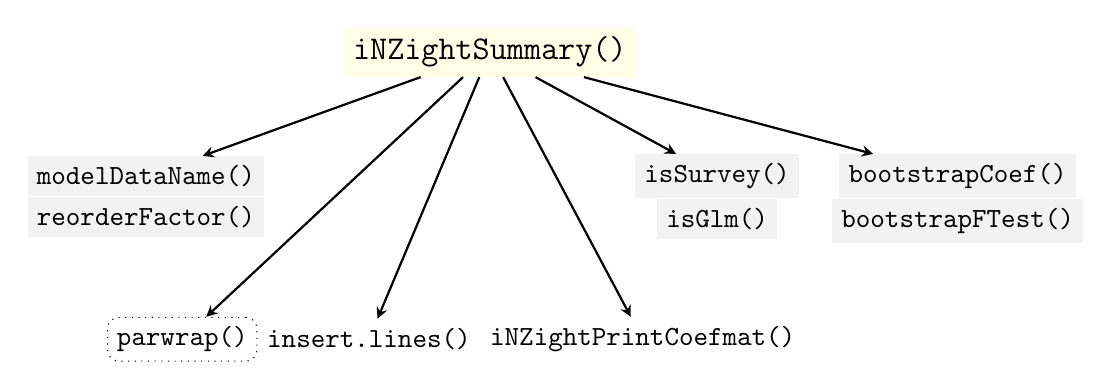
\begin{tikzpicture}
    \node(1)[main]{iNZightSummary()};
      \node(1-a)[other, below left=of 1]{modelDataName()};
        \node(1-a-a)[other, below=of 1-a, yshift=1cm]{reorderFactor()};
      \node(1-b)[other, right=of 1-a, xshift=3.7cm]{isSurvey()};
        \node(1-b-a)[other, below=of 1-b, yshift=1cm]{isGlm()};
      \node(1-c)[other, right=of 1-b, xshift=-0.5cm]{bootstrapCoef()};
        \node(1-c-a)[other, below=of 1-c, yshift=1cm]{bootstrapTTest()};
        \node(1-c-b)[other, below=of 1-c, yshift=1cm]{bootstrapFTest()};
      \node(1-d)[within, below right=of 1-a-a, xshift=-3cm]{parwrap()};
      \node(1-e)[f, right=of 1-d, xshift=-1cm]{insert.lines()};
      \node(1-f)[f, right=of 1-e, xshift=-1cm]{iNZightPrintCoefmat()};
    \draw[arrow](1)--(1-a);
    \draw[arrow](1)--(1-b);
    \draw[arrow](1)--(1-c);
    \draw[arrow](1)--(1-d);
    \draw[arrow](1)--(1-e);
    \draw[arrow](1)--(1-f);
  \end{tikzpicture}
  \caption{\texttt{summary.R}}
\end{figure}

\end{document}